\lecture{9}{fri 10 sep 10:50}{Taxes}
\section{Taxes}
\begin{definition}
    Taxes are a sum of money demanded by the government to support the government itself, as well as specific facilities or services. It is paid by \textbf{taxpayers} or people who pay tax to national, state government, or municipal government.
\end{definition}
There are 4 types of taxes:
\begin{itemize}
    \item Income
    \item Payroll
    \item Sales
    \item Excise tax - Focused alot in Micro
\end{itemize}
 These taxes follow 3 types of structure: progressive, proportional, and regressive taxes. In AP Micro we focus alot on \textbf{Excise Tax}.
 \begin{definition}
     Excise tax are taxes paid when purchases aer made on specific goods. It is a per unit tax, and is on a narrow range of products. It is more burdensome than a sales tax, and is often a higher percent of the retail price. 
 \end{definition}

 Now that we know what Excise tax is, lets go back to the structures and learn what they are.
 \begin{itemize}
     \item Progressive:
         \begin{itemize}
             \item \% of income paid in taxes increases as income increases
             \item Income tax
         \end{itemize}
     \item Proportional: 
         \begin{itemize}
             \item \% of income paid in taxes remains constant
             \item Flat tax
             \item Payroll tax for Medicare
         \end{itemize}
     \item Regressive:
         \begin{itemize}
             \item \% of income paid in taxes decreases as income increases
             \item Sales tax, higher income houses spend lower of their incomes. 
         \end{itemize}
 \end{itemize}

 Taxes reduce consumer and producer surplus, as both buyers pay more and sellers receive less. This is considered a wedge, and causes the quantity sold to fall below the natural market equilibrium. The \textbf{Total Werlfare} declines because the market shrinks, unless the government is correcting a market failure. 
 With a tax, the \textbf{Total Surplus} becomes the CS + PS + Tax Revenue. Since the market shrinks, the total surplus declines which ends up being the DWL. The size of DWL is determined by the \textbf{ELASTICITY}. 
 The greater the elasticity of demand and supply:
\begin{itemize}
    \item The larger the decline in equilibrium quantity
    \item The greater the DWL of a tax
    \item[!] Dont worry, we will cover elasticity alot more later
\end{itemize}

The tax causes some buyers and sellers to drop out of the market, as it increases the amount a consumer has to pay and decrease the amount a seller will receive. Lets look at a graph that demonstrates this idea in a bit more detail. 

\begin{figure}[H]
\begin{center}
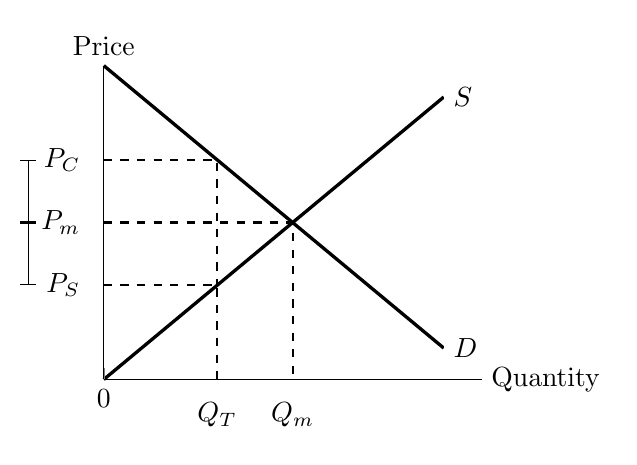
\begin{tikzpicture}
\begin{axis}[
scale=0.7,
xmin = 0, xmax = 10,
ymin = 0, ymax = 10, 
axis lines* = left,
xtick = {0}, ytick = \empty,
axis on top, 
clip = false,
]

\addplot[color = black, very thick] coordinates {(0,10) (9,1)};
\addplot[color = black, very thick] coordinates {(0,0) (9,9)};

\addplot[color = black, dashed, thick] coordinates {(0,5) (5,5) (5,0)};
\addplot[color = black, dashed, thick] coordinates {(0,3) (3,3) (3,0)};
\addplot[color = black, dashed, thick] coordinates {(0,7) (3,7) (3,3)};

\node [right] at (current axis.right of origin) {Quantity};
\node [above] at (current axis.above origin) {Price};
\node [left = 5pt] at (0,5) {$P_m$};
\node [below = 5pt] at (5,0) {$Q_m$};
\node [right, fill = white] at (9,1) {$D$};
\node [right, fill = white] at (9,9) {$S$};
\node [below = 5pt] at (3,0) {$Q_T$};
\node [left = 5pt] at (0,3) {$P_S$};
\node [left = 5pt] at (0,7) {$P_C$};
\draw[|-|] (-2, 5) to (-2, 7);
\draw[|-|] (-2, 3) to (-2, 5);

\end{axis}
\end{tikzpicture}
\caption{Tax affects welfare}
\label{fig:welfare}
\end{center}
\end{figure}

This just shows the tax wedge, and how that contributes to DWL. In this scenario, the government would benefit as it collects the tax revenue to provide public goods and services. The line between $P_C$ and $P_S$ is the total tax wedge. Buyers pay more, sellers recieve less, and the quantity with tax decreases. 

Whenever you make a graph, you want to place it onto the Supply curve, since tax is comparable to a input cost.
\textbf{How to graph a per unit tax:}
\begin{enumerate}[label=Step \arabic*:]
\item Draw a market model graph that is labeled
\item Identify the value of the tax. Example 2.00 dollars per unit
\item Apply the tax to the graph, by drawing a new supply to the left. \textbf{DON'T DRAW ARROWS}. This is not a true shift, but a graph technique to show a tax 
\item Label Qtax and now there are two prices Ps and Pd. The price is always determined by what consumers are willing to pay
\item Read the graph - New price is Qm + value of tax
\end{enumerate}

Lets do an example with sweaters if they were imposed a 50c excise tax. 

\begin{figure}[!h]
\begin{center}
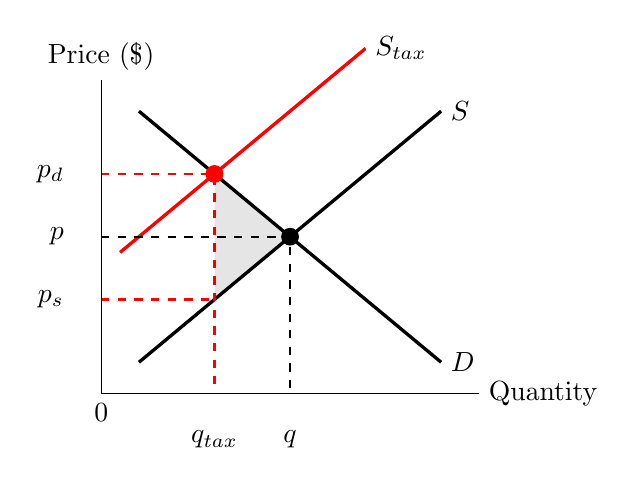
\begin{tikzpicture}
\begin{axis}[
scale=0.7,
xmin = 0, xmax = 10,
ymin = 0, ymax = 10, 
axis lines* = left,
xtick = {0}, ytick = \empty,
axis on top, 
clip = false,
]

\addplot[color = black, very thick] coordinates {(1,9) (9,1)};
\addplot[color = black, very thick] coordinates {(1,1) (9,9)};
\addplot[color = red, very thick] coordinates {(0.5,4.5) (7,11)};
%\addplot[color = blue, very thick] coordinates {(2,10) (10,2)};
% Dashed Lines
\addplot[color = black, dashed, thick] coordinates {(0,5) (5,5) (5,0)};
\addplot[color = red, dashed, thick] coordinates {(0,7) (3,7) (3,0)};
\addplot[color = red, dashed, thick] coordinates {(0,3) (3,3)};
% Points
\addplot[color = black, mark = *, only marks, mark size = 3pt] coordinates {(5,5)};
\addplot[color = red, mark = *, only marks, mark size = 3pt] coordinates {(3,7)};
% Fill
\fill[black, opacity = 0.1] (3,7) -- (5,5) -- (3,3);
% Labels
\node [right] at (current axis.right of origin) {Quantity};
\node [above] at (current axis.above origin) {Price (\$)};
\node [left = 10pt] at (0,5) {$p$};
\node [below = 10pt] at (5,0) {$q$};
\node [left = 10pt] at (0,7) {$p_d$};
\node [left = 10pt] at (0,3) {$p_s$};
\node [below = 10pt] at (3,0) {$q_{tax}$};
\node [right, fill = white] at (9,1) {$D$};
\node [right, fill = white] at (9,9) {$S$};
\node [right, fill = white] at (7,11) {$S_{tax}$};
%\fill[black, opacity = 0.1] (3,7) -- (5,5) -- (3,3);

\end{axis}
\end{tikzpicture}
\caption{Sweaters with tax}
\label{fig:sweaters}
\end{center}
\end{figure}

The DWL is a cost to society as a whole that is generated by an economically inefficient allocating of resources within the market. Mutually beneficial transactions do not occur. Allocative efficiency is reduced; it does not reach its maximum level. 

The effect of a tax is that the government will obtain revenue from it, to calculate the revenue it is just, 
\[
T * Q = \text{the government's tax revenue}
.\] 
where 
\begin{description}
    \item[T] = Size of the tax
    \item[Q] = Quantity of good sold
\end{description}

Its important to understand that as the size of the tax rises, the revenue grows \textbf{up to a certain point}. The increase in tax can cause the size of the market to decrease lowering the revenue. 
